\chapter{Gestão dos Conhecimentos}

Neste capítulo, serão apresentadas as tecnologias que serão utilizadas para o desenvolvimento do projeto, e o motivo da utilização, além de uma contextualização de cada uma delas.

% \section{Machine Learning}

% \textit{Machine Learning} é uma área da Ciência da Computação que estuda o desenvolvimento de algoritmos capazes de aprender a executar uma tarefa com sua própria experiência, sem
% a necessidade de programar explicitamente todas as regras para cada tarefa específica \cite{cerri2019aprendizado}. A complexidade do aprendizado de máquina reside no fato de que o sucesso dos algoritmos depende da qualidade e da quantidade dos dados, além da escolha adequada dos modelos e técnicas \cite{DBLP:journals/cacm/Domingos12}.

% Existem três principais paradigmas em aprendizado de máquina: Aprendizado Supervisionado, Não Supervisionado e por Reforço.

% No Aprendizado Supervisionado, o modelo é treinado com dados rotulados, onde, para cada exemplo apresentado ao algoritmo, há uma resposta correta associada. Nesse caso, o algoritmo aprende a relacionar entradas às saídas desejadas, buscando generalizar esse conhecimento para realizar previsões precisas sobre novos dados.

% Por outro lado, no Aprendizado Não Supervisionado, os dados fornecidos ao algoritmo não possuem rótulos. O objetivo é identificar padrões ou estruturas ocultas nos exemplos sem orientação explícita. Algoritmos comuns buscam agrupar dados semelhantes, formando agrupamentos ou \textit{clusters}.

% Já no Aprendizado por Reforço, o algoritmo interage diretamente com um ambiente, recebendo recompensas ou punições conforme suas ações. As recompensas reforçam comportamentos desejáveis, enquanto as punições servem para impedir as ações fracassadas. O objetivo é maximizar a recompensa acumulada ao longo do tempo, desenvolvendo uma política ótima de comportamento. O algoritmo \textit{Q-Learning} é um dos mais conhecidos e utilizados desse paradigma \cite{watkins1989learning}.

% É importante levantar que os modelos de Processamento de Linguagem Natural abordados neste trabalho, como o GloVe e o FastText, utilizam o aprendizado não supervisionado para seu treinamento.

\section{Word Embeddings}

No processamento de linguagem natural, word embeddings são representações vetoriais que mapeiam palavras para um conjunto de vetores de valores reais em um espaço N-dimensional predefinido, de modo que palavras que possuem significado semântico, contextual e sintático próximas no vocabulário sejam representadas por vetores próximos nesse espaço \cite{mikolov2013efficient}. Essas representações são aprendidas por meio de algoritmos de \textit{machine learning} que são gerados a partir de seu contexto.

\begin{figure}[h!]
    \centering
    
    \label{fig:relacao-lineares-palavras}
    \caption{Relações lineares entre palavras.}
    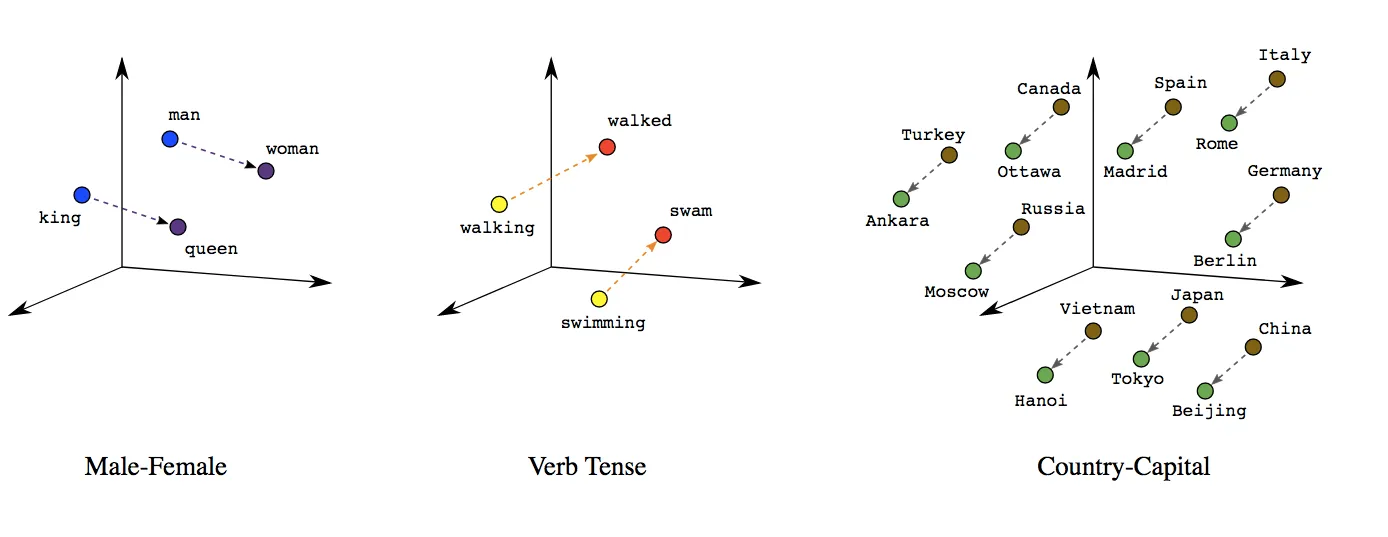
\includegraphics[width=1\textwidth]{figs/relacao-palavras.jpg} 
    
    Fonte: \cite{duzzi2023}
\end{figure}

Inicialmente, técnicas como \textit{Bag of Words} (BoW) e TF-IDF eram amplamente utilizadas, baseando-se em vetores de alta dimensionalidade, nos quais cada palavra era representada como um índice isolado, sem considerar semelhanças semânticas entre diferentes termos. Apesar de sua simplicidade, esses métodos apresentavam limitações expressivas, especialmente na incapacidade de capturar relações semânticas ou contextuais entre as palavras \cite{mikolov2013efficient}.

Existem diversas abordagens para a obtenção de representações vetoriais de palavras, mas a maneira mais popular é treinando redes neurais, como é o caso do famoso \textit{Word2vec}, modelo de aprendizado de máquina desenvolvido por \citeonline{mikolov2013efficient} em 2013. Esse algoritmo utiliza redes neurais rasas para gerar embeddings.

\section{Word2Vec}

O modelo Word2Vec pode ser treinado a partir de duas arquiteturas possíveis: \textit{Continuous Bag-of-Words} (CBOW) e \textit{Skip-Gram}. O CBOW prevê uma palavra com base em seu contexto, enquanto o Skip-Gram prevê o contexto a partir de uma palavra. Por exemplo, a expressão vetorial “vetor(‘rei’) - vetor(‘homem’) + vetor(‘mulher’)” resulta em um vetor próximo ao vetor de “rainha”, evidenciando a captura das relações semânticas \cite{MikolovYZ13}.

A arquitetura do Word2Vec é baseada em uma rede neural rasa composta por três camadas: entrada, oculta e saída. Na camada de entrada, cada palavra é representada por um vetor one-hot, que é então transformado em um vetor denso na camada oculta por meio de uma matriz de pesos. Essa matriz de pesos é, na verdade, o que constitui os embeddings de palavras aprendidos pelo modelo \cite{Rong14}.

\begin{figure}[h!]
    \centering
    
    \label{fig:representacao-modelos-w2v}
    \caption{Representação dos modelos Word2Vec.}
    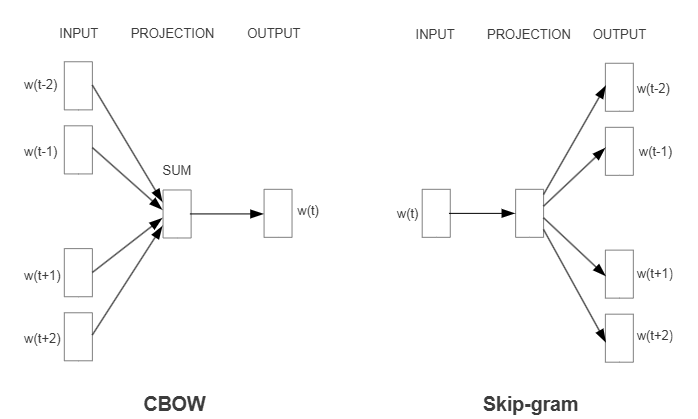
\includegraphics[width=1\textwidth]{figs/representacao-modelos-w2v.png} 
    
    Fonte: \cite{mikolov2013efficient}
\end{figure}

Já a camada de saída utiliza outra matriz de pesos para prever as palavras de contexto, no modelo Skip-Gram, ou a palavra central, no modelo CBOW, aplicando uma função \textit{softmax} para gerar uma distribuição de probabilidade sobre o vocabulário. O treinamento da rede ajusta os pesos de ambas as matrizes para minimizar a diferença entre as previsões e as palavras reais observadas no corpus.

\section{GloVe}

O \textit{GloVe}, sigla para \textit{Global Vectors } (Vetores Globais), desenvolvido per \citeonline{pennington2014glove}, é um algoritmo de aprendizado não supervisionado usado para criar word embeddings. Sua principal inovação foi combinar o melhor de duas abordagens anteriores: a eficiência estatística global dos métodos baseados em contagem, como a análise de coocorrência em todo o texto, e o desempenho superior em tarefas de analogia dos métodos preditivos baseados em contexto local, como o Word2Vec.

O GloVe opera construindo uma matriz global de coocorrência de palavras e, em seguida, treina um modelo de regressão ponderada para aprender vetores cujo produto escalar se aproxima do logaritmo da probabilidade de coocorrência dessas palavras. O resultado são embeddings que capturam de forma eficaz as relações semânticas e sintáticas complexas.

\section{FastText}

Técnicas de incorporação de palavras, como Word2Vec e GloVe, fornecem representações vetoriais únicas para cada palavra do vocabulário, negligenciando a estrutura morfológica interna desses termos. Essa abordagem é uma limitação significativa para línguas morfologicamente ricas, pois ignora as relações sintáticas e semânticas evidentes na formação das palavras (prefixos, sufixos e radicais).

Para superar essa limitação, o \textit{FastText}, uma extensão do modelo Word2Vec, enriquece as representações vetoriais usando informações em nível de caractere. O FastText aprende embeddings para n-gramas de caracteres (subpartes da palavra) e representa uma palavra como a soma ou a média dos vetores de seus n-gramas constituintes. Assim como o antecessor, ele também utiliza as arquiteturas CBOW e Skip-Gram para o treinamento.

A principal vantagem dessa abordagem é a capacidade de lidar com palavras fora do vocabulário (\textit{Out-of-Vocabulary} — OOV). Modelos como Word2Vec ou GloVe não conseguem gerar vetores para palavras que não estavam presentes nos dados de treinamento. O FastText, ao contrário, pode construir a representação de uma palavra OOV simplesmente somando os vetores de seus n-gramas de caracteres, permitindo-lhe inferir o significado de termos novos ou raros com base em sua composição. \cite{bojanowski-etal-2017-enriching}

\section{Tecnologias}

\subsection{Python}

\textit{Python} é uma linguagem de programação de alto nível, criada por Guido van Rossum em fevereiro de 1991. A linguagem foi desenvolvida com uma sintaxe clara e legível, que se assemelha à linguagem humana. Além disso, o Python é uma linguagem interpretada e de tipagem dinâmica, o que significa que as variáveis não precisam ter seu tipo explicitamente declarado, facilitando a curva de aprendizado e o desenvolvimento de aplicações.

Em 2024, Python se tornou a linguagem de programação mais utilizada no \textit{GitHub}, ultrapassando \textit{JavaScript} pela primeira vez desde o início da plataforma\footnote{\url{https://github.blog/news-insights/octoverse/octoverse-2024/}, acessado em \today.}. Essa marca só foi possível de ser alcançada devido ao aumento de projetos relacionados à Inteligência Artificial, ciência de dados e aprendizado de máquina, áreas nas quais Python é amplamente adotado devido à extensa variedade de bibliotecas disponíveis. 

% Por esse mesmo motivo, Python foi escolhido como a linguagem de programação para este projeto, garantindo uma implementação alinhada com as tendências atuais do desenvolvimento de aprendizado de máquina.

\subsection{Gensim}

O \textit{Gensim} é uma biblioteca \textit{open-source} em Python projetada para representar documentos como vetores semânticos de maneira eficiente, facilitando o processamento e análise de textos não estruturados. Utilizando algoritmos de aprendizado não supervisionado, como Word2Vec e FastText, o Gensim é capaz de descobrir automaticamente a estrutura semântica dos documentos, analisando padrões de coocorrência estatística em grandes corpora de texto. Esses modelos transformam textos em representações vetoriais, permitindo consultas de similaridade semântica entre palavras, frases e documentos, o que promove uma análise mais profunda e automatizada do conteúdo textual. \cite{rehurek_lrec}

% O Gensim foi utilizado no projeto para carregar o modelo de embending e fazer as comparações.

\subsection{Playwright}
O \textit{Playwright} é um framework de código aberto mantido pela \textit{Microsoft}, desenvolvido para a automação de navegadores e a execução de testes de ponta-a-ponta (\textit{end-to-end}). Seu principal diferencial é a capacidade de controlar os três principais motores de renderização, \textit{Chromium}, \textit{Firefox} e \textit{WebKit}, por meio de uma API única e unificada. Essa abordagem permite que desenvolvedores e analistas de qualidade escrevam um único \textit{script} de teste e o executem de forma consistente em todos os principais navegadores. O framework oferece suporte a diversas linguagens, como Python, JavaScript, Java e C\#.\footnote{\url{https://playwright.dev/docs/intro}, acessado em \today.}

% \subsection{Numpy}
% NumPy é o pacote fundamental para computação científica em Python. É uma biblioteca Python que fornece um objeto de array multidimensional, vários objetos derivados (como arrays e matrizes mascaradas) e uma variedade de rotinas para operações rápidas em arrays, incluindo operações matemáticas, lógicas, manipulação de formas, ordenação, seleção, entrada/saída, transformadas discretas de Fourier, álgebra linear básica, operações estatísticas básicas, simulação aleatória e muito mais.\footnote{\url{https://numpy.org/doc/stable}, acessado em \today.

\subsection{Hugging Face Hub}
O Hugging Face Hub é uma plataforma com mais de 2 milhões de modelos, 500 mil conjuntos de dados e 1 milhão de demonstrações, na qual as pessoas podem colaborar facilmente em seus fluxos de trabalho de aprendizado de máquina. O Hub funciona como um local central onde qualquer pessoa pode compartilhar, explorar, descobrir e experimentar com aprendizado de máquina de código aberto.\footnote{\url{https://huggingface.co/docs/hub/index}, acessado em \today.}